\documentclass[a4paper]{article}
\usepackage{graphicx}
\usepackage{epstopdf}
\usepackage{mcode}
\usepackage{style}
\usepackage{float}
\title{Laboration - Solid state physics\\ The bipolar junction transistor}

\author{Alexander Najafi \\ Linus Hellman}

\date{2014-05-10}

\begin{document}

\maketitle
\thispagestyle{empty}
\newpage

\tableofcontents
\newpage
\section{Introduction}
The purpose of this lab is to gain a better understanding of the bipolar transistor characteristics. By altering the different potentials over the three sections of the transistor we hope to establish a connection between them and in that way learn to understand it. The lab mainly consists in three parts, measuring the capacitor in a pn-junction, measuring the current through a pn-junction and measuring the currents through a bipolar npn-transistor.

In the first part we are studying the capacitor in the pn-junction. The total capacitance that is found in a pn-junction actually consists of capacitors from two different origins, one is called junction capacity and the other one is called diffusion capacity. The junction capacity exist because of that the depletion area has a very high resistance so that when the n and p sections has voltage difference the junction can be seen as a capacitor. The second capacitance origins in the neutral part of the p-doped section. When the pn-junction is forward biased there is an increase of minority charge carriers and the amount of these are directly proportionate to the forward biased charge. Since the definition of capacitance is $C=\frac{Q}{U}$ and since that is exactly what is occurring here it's perceived as a capacitance. Expressions for these capacitances are as follows.

\begin{equation}
C_j=\sqrt{\frac{A^2{\cdot}\epsilon_r{\cdot}\epsilon_0{\cdot}e{\cdot}N_A}{2(U_{bi}-U_A)}}
\end{equation}
\begin{equation}
C_{diff}=\frac{e{\cdot}n_{p_0}{\cdot}A{\cdot}W_p}{2{\cdot}U_t}e^{(\frac{U_a}{U_t})}
\end{equation}

The total capacitance for the pn-junction is simply the sum of these two capacitances. The characteristics of these can be seen in the picture below.

\begin{figure}[H]
\centering
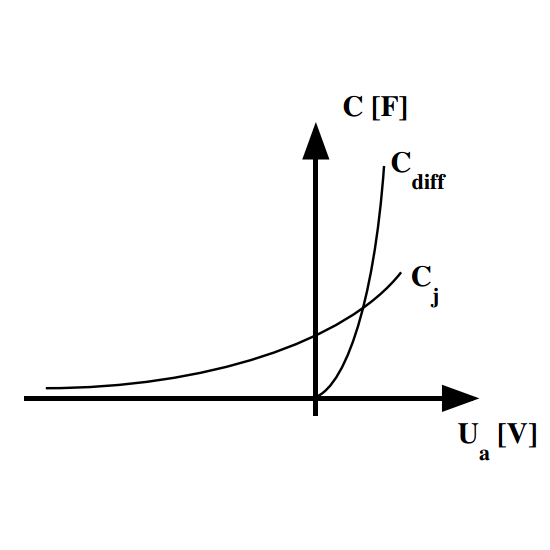
\includegraphics[scale=0.3]{capp.png}
\caption{The two capacitances that can be seen in a pn-junction}
\label{capp}
\end{figure}

In the next part the current through a pn-junction where to be analysed. The current characteristics for a pn-junction can be explained by looking at it's construction. The junction basically consists of two blocks one that is doped with donors which is called n-doped and one that is doped with acceptors that is called p-doped. The n-doped block has an excess of electrons and the p-doped has an excess holes. When these two blocks is put together the electron and the holes starts to recombine this creates the highly resistive depletion area between the two blocks. The depletion area may be altered with an outside voltage, if the junction where to be forward biased then the depletion area will shrink leading to a smaller resistance thus a bigger current. If the junction where to be reversed biased then it will lead to a bigger resistance and a smaller current. In a way this can be seen as a variable resistance that depends on the voltage over the junction. This nexus is pictured below where a) is without a outside voltage, b) is reversed biased and c) is forward biased.

\begin{figure}[H]
\centering
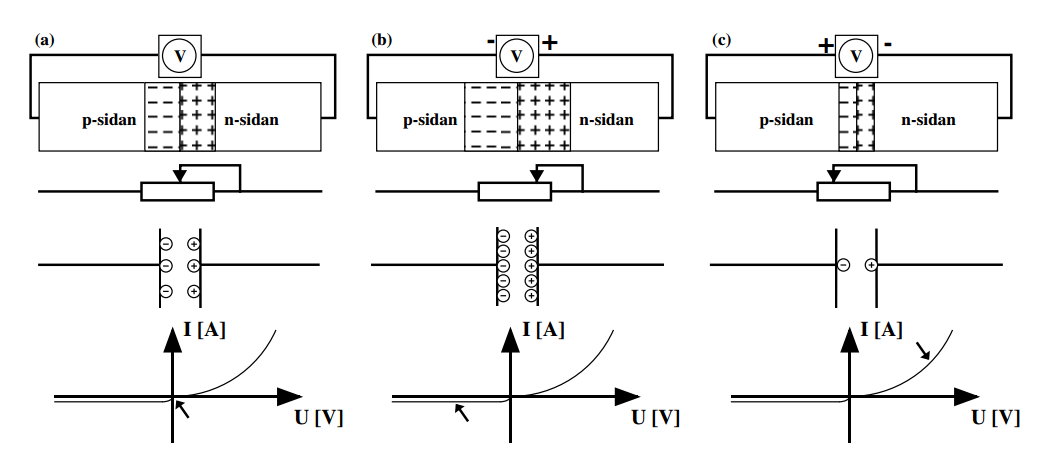
\includegraphics[scale=0.3]{diodeeffect.png}
\caption{The diode effect}
\label{diode}
\end{figure}

The final part in this lab consisted in measuring the characteristics of a BJT (bipolar junction transistor). As in the second part it's easier to explain how the transistor work by looking at how it's constructed. The three main sections of the transistor is the base, the collector and the emitter. To get the transistor to it's active mod (the most commonly used mod) the base-collector is put in a reversed biased state creating an electric field in the depletion area. The base-emitter junction is then put in a forward biased state. This causes electrons from the base-emitter junction to diffuse into the electric field of the base-collector junction and is accelerated towards the collector. This can be seen as a current from the collector to the emitter and is called $I_c$. The size of this current is controlled by the base-emitter voltage. An ideal BJT would climb up to it's maximum $I_c$ for an arbitrary value of the base-emitter voltage and then stay constantly on this level disregarding the change of the collector-emitter voltage. But in a real BJT there is a parasite resistance between the collector and the emitter causing the collector-emitter current to increase slightly when the collector-emitter voltage is increased. This is called the Early effect.

\section{Result}
\subsection{Pn-junction UI}
The following graph was plotted for the pn-junction U-I characteristics. See the measured data in the appendix together with the matlab-code. 
\begin{figure}[H]
	\centering
	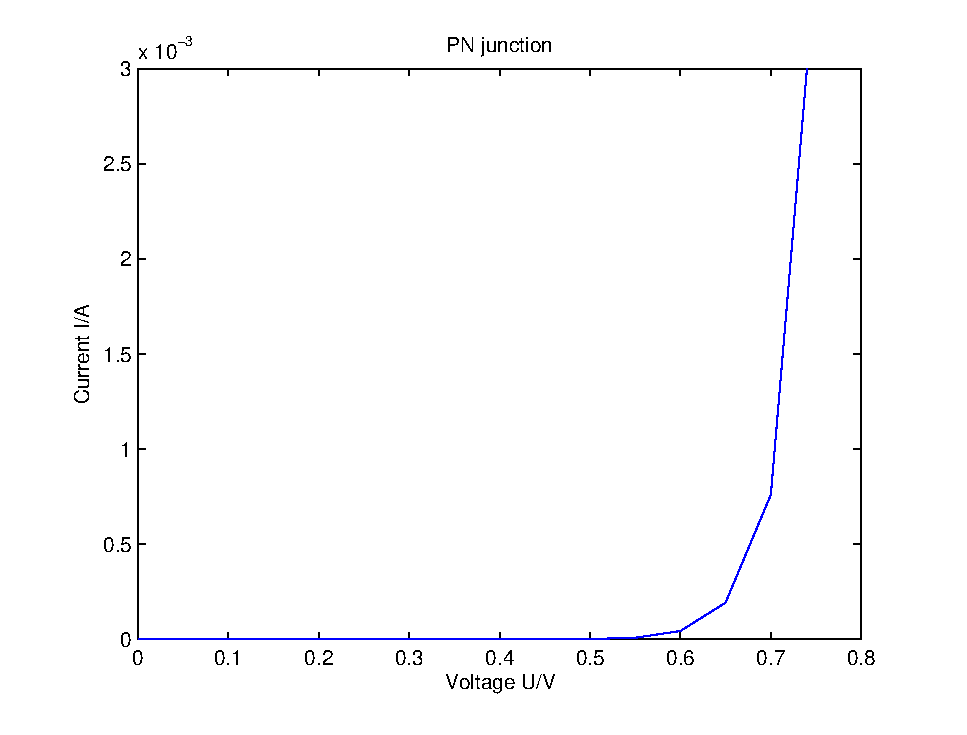
\includegraphics[width=0.7\textwidth]{pn_ui.eps}
	\caption{U-I characteristics for the pn-junction.}
	\label{pn_ui}
\end{figure}

\subsection{PN junction capacitance}
The following graph was plotted using the measured data in the appendix for the capacitance in the PN junction. See appendix for values and matlab-code. 
\begin{figure}[H]
	\centering
	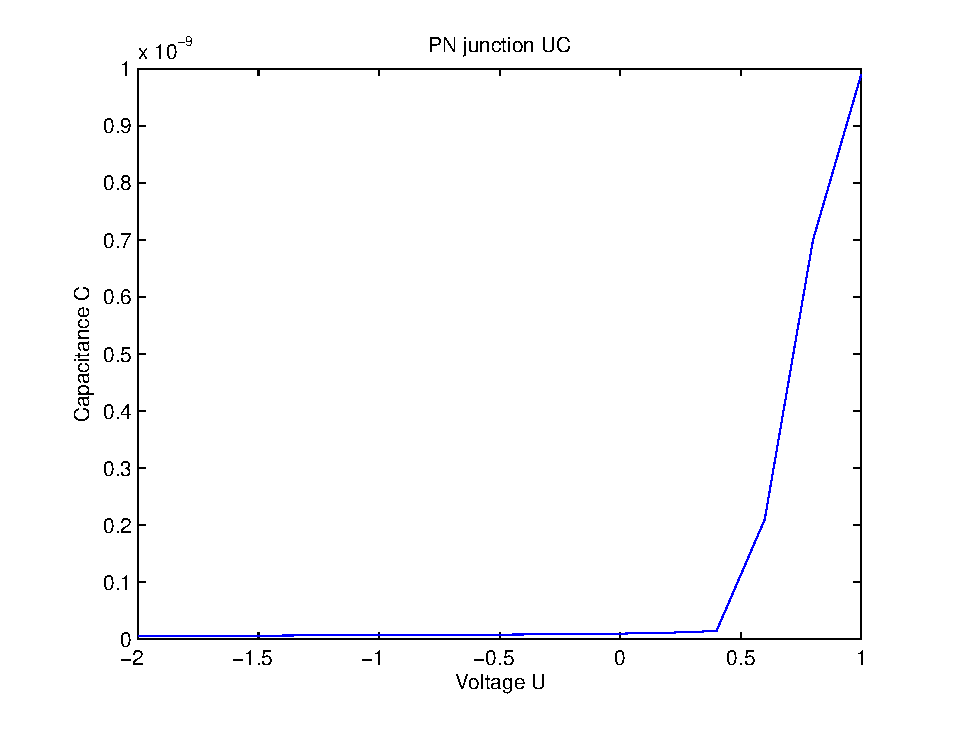
\includegraphics[width=0.7\textwidth]{pn_cap.eps}
	\caption{C-U characteristics for the pn-junction.}	
	\label{pn_cap}
\end{figure}

\subsection{NPN transistor}
The following graphs were plotted for the current in the npn transistor. The early voltage was calculated to 34V using matlab. See the appendix for values and matlab-code.
\begin{figure}[H]
	\centering
	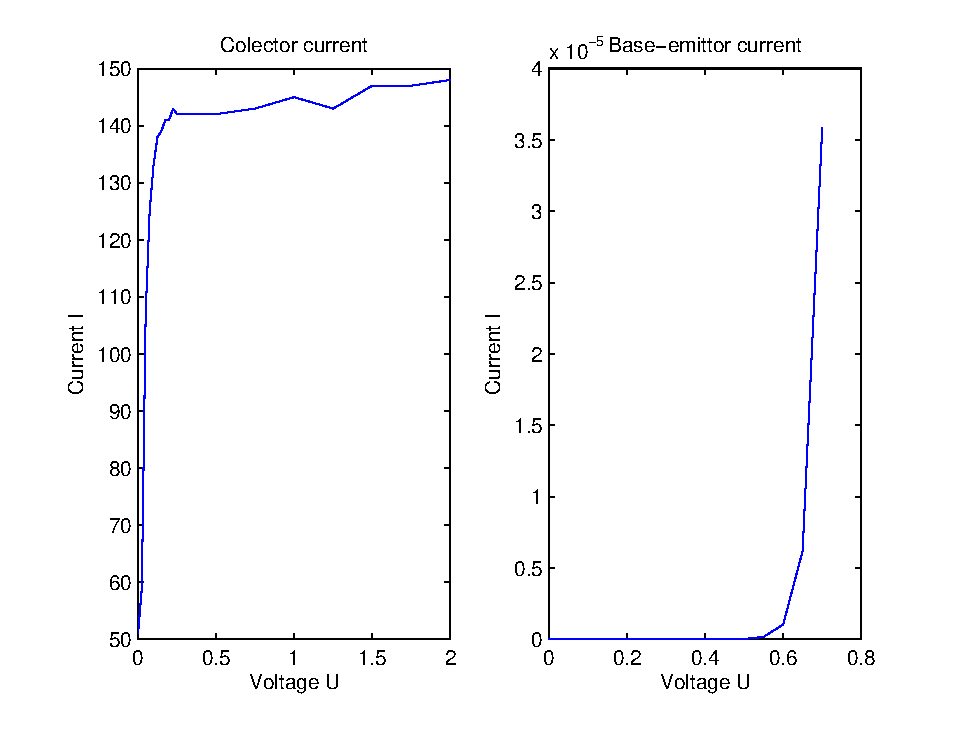
\includegraphics[width=0.85\textwidth]{npn.eps}
	\caption{Voltage to current characteristics for the NPN transistor. The collector current to the left and the base-emitter current to the right.}	
	\label{npn}
\end{figure}

\newpage
\section{Analysis of the result}
\subsection{PN junction UI}
In figure \ref{pn_ui} the current to voltage ratio is plotted from the measured values. Since this is a pn-junction it is expected to behave like a normal diode. In the graph it is clear that the current through the pn-junction is zero until it the voltage over the junction reaches about 0.7V. This value of the forward voltage is expected and is about the same for all pn-junctions.

The forward voltage exists since...

\subsection{PN junction capacitance}


\subsection{NPN transistor}
As you can see to the left in figure \ref{npn} an increasing voltage from zero to about 0.25 volts results in a substantially increase in the collector current. The current doesn't increase to infinity and beyond though. The current that flows through the transistor is dependent on the current that the power source can deliver. The steep increase in current stops since there are no more electrons that can diffuse from the emitter through the base to the collector in the transistor.

To calculate the early voltage a linear function was approximated to the eleven largest values that were measured. To find the approximation function $p(U) = ax + b$ polyfit was used in matlab (see appendix). Using the function and calculating $p(U) = 0 => x = \frac{b}{a}$ the early voltage was found to be $\frac{139,9}{4,1} \approx 34V$.

The right graph in figure \ref{npn} shows the current that flows from the base to the emitter. Since this is a pn-junction it was expected that the current to voltage graph would look like a diodes graph, which it does. The forward voltage for the pn-junction is shown in the graph to be about 0.6-0.7 V which is normal value expected for a diode.

\newpage
\appendix
\section{Matlab code}
\subsection{PN junction UI}
\lstinputlisting{pn_current.m}
\subsection{PN junction capacitance}
\lstinputlisting{pn_cap.m}
\subsection{NPN current}
\lstinputlisting{npn.m}

\end{document}
